\chapter{Implementation}
\label{chap:implementation}

In this chapter, we investigate how to connect the computer vision algorithms described in Chapter \ref{chap:algorithms} to obtain a program solving the task of 3D reconstruction on a mobile phone. 
The result of this work is an Android application that allows the user to take photos with phone's camera, browse them and pick a pair of images to reconstruct. 
The reconstructed scene is then visualized in 3D using OpenGL~ES.
Recall the properties of the input pair of photos described in Section~\ref{prob}.
(An example of a suitable pair of images is shown in Figure \ref{fig:input_samples}.)

The following are the main obstacles we are faced with when trying to solve this problem: 
\begin{itemize}
\item mobile phones typically have a limited computational power, 
\item they also have limited operational memory, 
\item most importantly, the optical properties of cameras included in a typical mobile phone are of mediocre quality at best. 
\end{itemize} 
The last property is particularly troublesome for us, since it implies -- among other problems -- that the captured image is defomed by an unknown non-linear transformation. 
% This is an issue often encountered in professional-grade cameras as well. 
% However, in these cases, this distortion can be efficiently estimated and accounted for since it typically behaves in a constrained manner. 
% For cheap mobile phone cameras, this is not possible and thus we have to keep in mind that 
This implies that the model of projective camera and the epipolar constraints discussed in Section \ref{sec:projective} are only a rough approximation. 
However, this significantly restricts the choice of computer vision algorithms to apply. 
For example, algorithms for the dense reconstruction problem are often heavily dependent on having a precise model of the epipolar constraints in the image pair. 

We solve this issue using a combination of sparse feature matching and the classical optical flow algorithm (both described in Chapter \ref{chap:algorithms}). 
Specifically, we employ the SURF algorithm since it has better computational efficiency compared with the SIFT algorithm.
Sparse feature matching can be successfully performed without any kind of epipolar constraint and therefore the inaccuracy of the camera model is not an issue. 
However, the resulting 3D information is only a sparse 3D point cloud reconstruction of the scene. 
Since this is insufficient for our purposes, we perform repeated optical flow calculation on pairs of neighborhoods of corresponding features. 

% The final section is devoted to technical aspects of the implementation. 

\section{Implementation outline}
\label{sec:impl_outline}
In the this section we describe our solution to the 3D reconstruction task and discuss why each utilized algorithm was chosen.
Let us begin with a brief overview of the algorithm, which is also depicted on Figure \ref{fig:impl}.
At first we find an initial estimate of the relative position of the pair of the input photos.
Then, we detect and match SURF features and use this information to compute the relative position more precisely. 
The next step is to detect a larger amount of SURF keypoints. 
The matching process uses the information of the relative position estimated in the previous step and thus can obtain significantly larger number of matches.
Finally, we compute the dense correspondences between the images using the Lucas-Kanade optical flow algorithm.
In the sections below, we discuss these steps in more detail. 

\vspace{0.5cm}
\begin{figure}[H]
\centering

\begin{subfigure}[b]{0.45\textwidth}
\centering
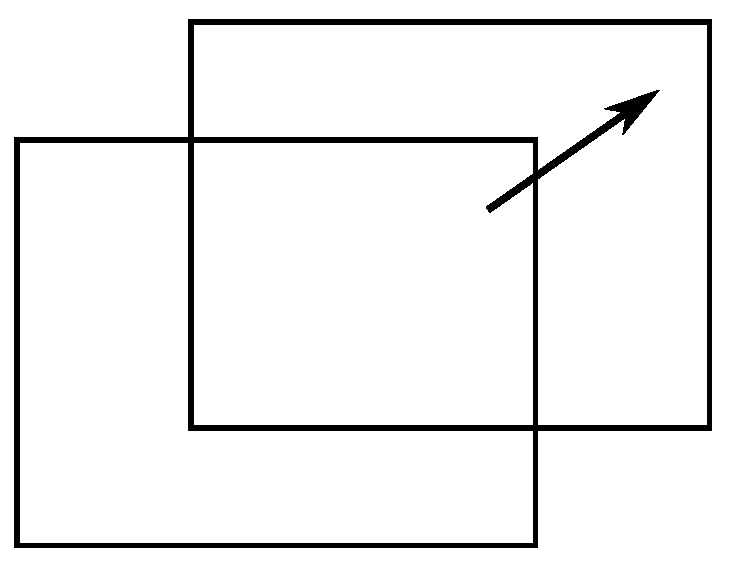
\includegraphics[width=3.8cm]{img/impl0.pdf}
\caption{An overall shift between the photos is computed.} \label{impl0}
\end{subfigure}
\hspace{0.5cm}
\begin{subfigure}[b]{0.45\textwidth}
\centering
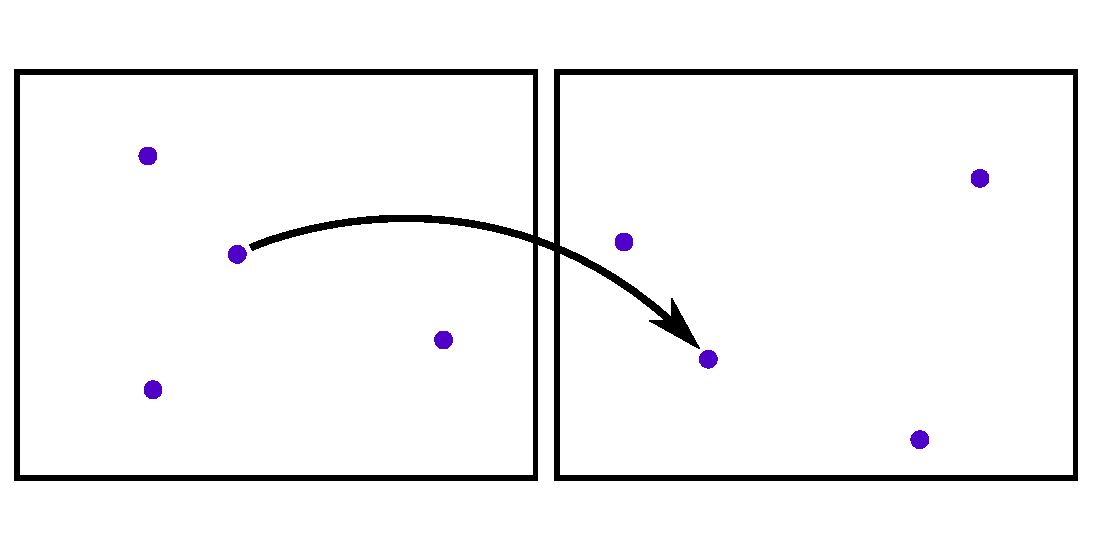
\includegraphics[width=6.5cm]{img/impl1.pdf}
\caption{Precise parameters of the translation are identified.} \label{impl1}
\end{subfigure}
\begin{subfigure}[b]{0.45\textwidth}
\centering
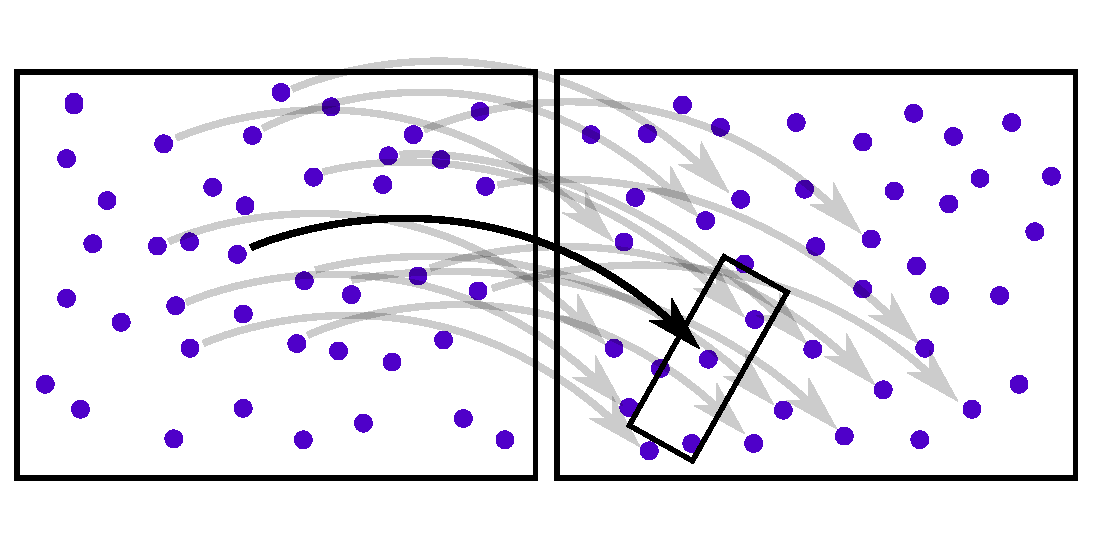
\includegraphics[width=6.5cm]{img/impl2.pdf}
\caption{Increasing the density of the SURF matches through local matching. Only features inside the rectangle are considered.} \label{impl2}
% Only features inside the bigger rectangle are considered, only features inside the smaller one are accepted as correspondences.
\end{subfigure}
\hspace{0.5cm}
\begin{subfigure}[b]{0.45\textwidth}
\centering
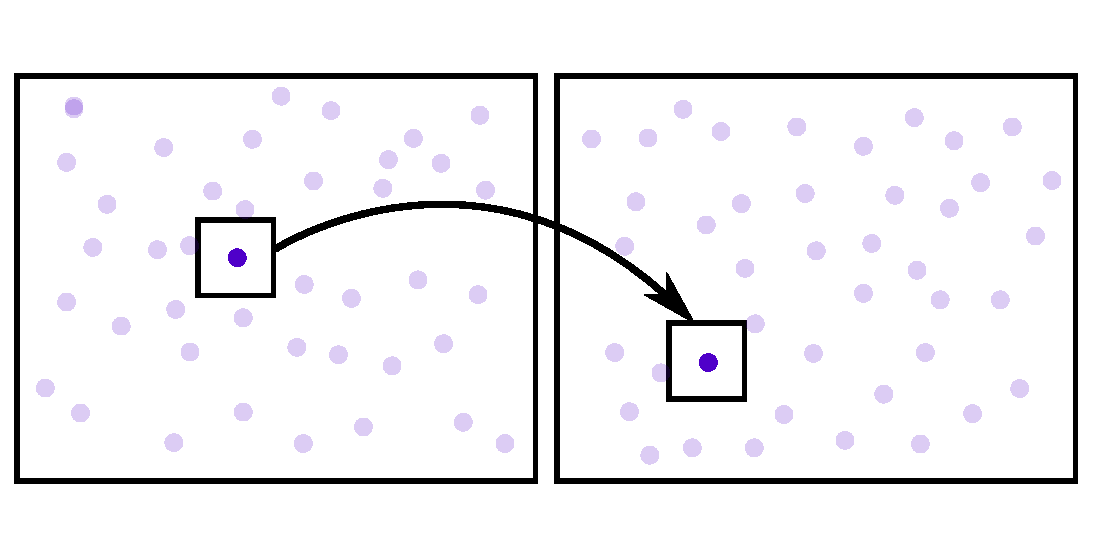
\includegraphics[width=6.5cm]{img/impl3.pdf}
\caption{Optical flow between neighbourhoods of corresponding features is computed to further improve the density of matched pixels.} \label{impl3}
\end{subfigure}

\caption[]{An illustration of the four main stages of our reconstruction pipeline.} 
\label{fig:impl}
\end{figure}
\vspace{0.5cm}

\subsection{Estimating the displacement vector}
The first step is illustrated on Figure~\ref{impl0}.
Finding the initial relative position of the pair of the images is implemented by using the sum of absolute differences (described in Section \ref{sec:metrics}).
For efficiency-related reasons, we begin by creating an image pyramid and find the overlap minimizing the sum of absolute differences in the lowest scale. 
We then use this position in a higher level of the pyramid, corresponding to a higher resolution. 
However, on this level, we only need to consider shifts by a small number of pixels. 
This upscaling continues until the image resolution is above a certain threshold. 
We call the resulting vector a \term{displacement vector}.
An example of the result of such computation is on Figure~\ref{emaover}.

\begin{figure}[H]
\centering
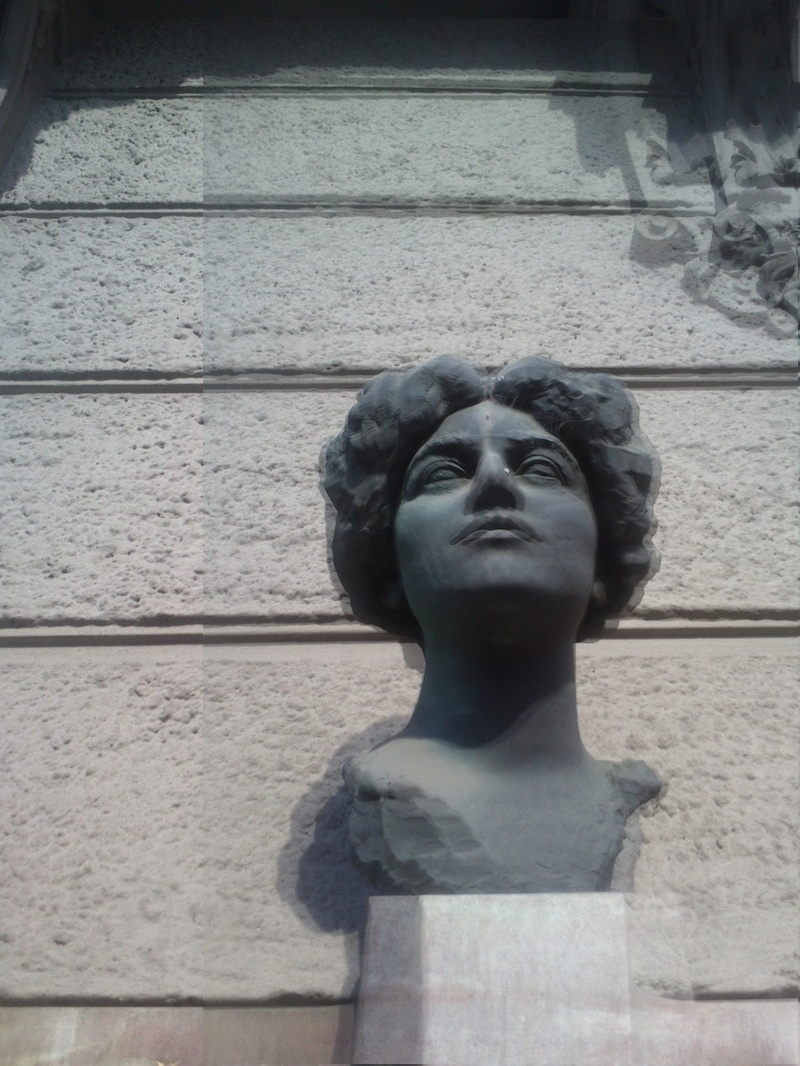
\includegraphics[width=5cm]{img/ema_overlap.png}
\caption{Two images blended together after being aligned using the minimization of the sum of absolute differences.}
\label{emaover}
\end{figure} 

\subsection{Improving the displacement vector estimate}
\label{sec:improving}

We now have a rough estimate of the relative position between the photos. 
Our aim now is to improve its precision.
This is done by considering SURF features detected with high values of the Hessian threshold. 
We consider these since their number is relatively low and they are highly repeatable. 

The basic approach would be to try matching every possible pair of features from the corresponding images. 
However, this method is very slow and unsuitable for our application. 
Therefore, we utilize the knowledge of the approximate relative position between the images in order to match these features efficiently.
We start by dividing the second image into square-shaped \term{buckets} of identical size and to each bucket we assign an array of features contained in it.
The situation is illustrated on Figures \ref{impl1} and \ref{emabuckets}.
When searching for a match for a feature in the first image, we estimate its corresponding position in the second image and consider a circular area around it. 
Then, we list the buckets intersecting it and iterate only through these features. 
Based on these matches, we estimate the displacement vector, giving us a more accurate relative position of the input pair of images.

\begin{figure}[h]
\centering
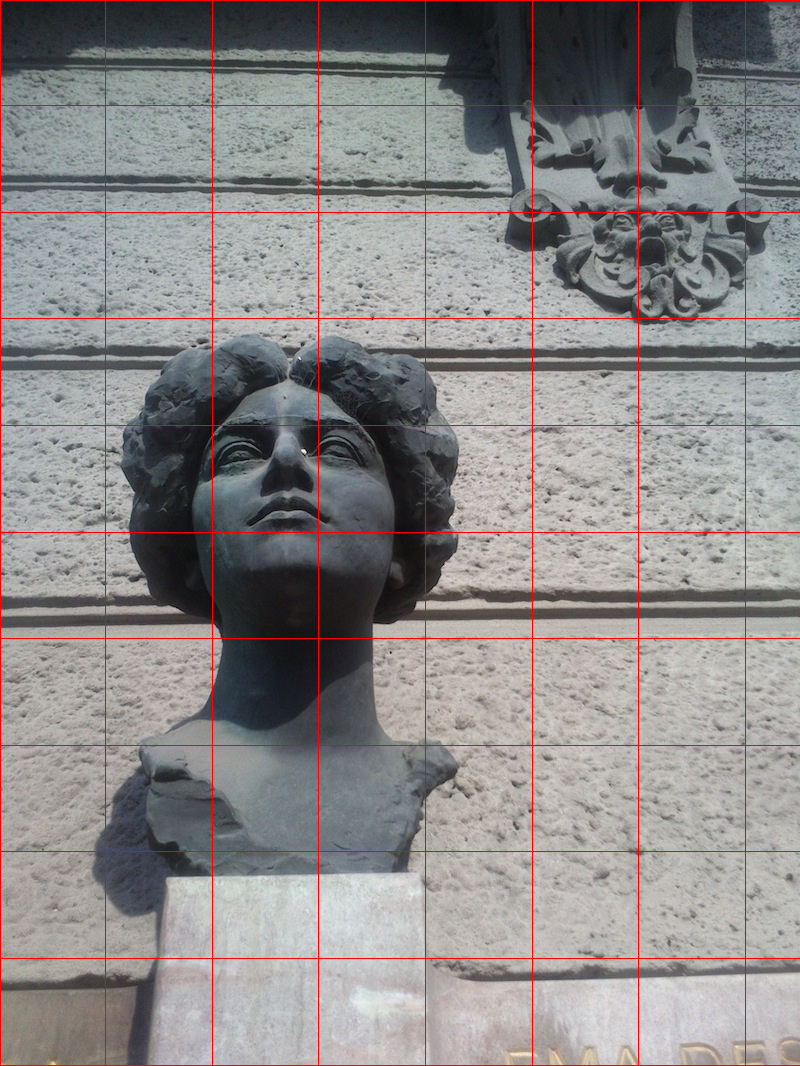
\includegraphics[width=5cm]{img/ema_buckets.png}
\caption{The partition of the second image in the dataset into buckets.}
\label{emabuckets}
\end{figure} 

% \begin{figure}[H]
% \centerline{
% 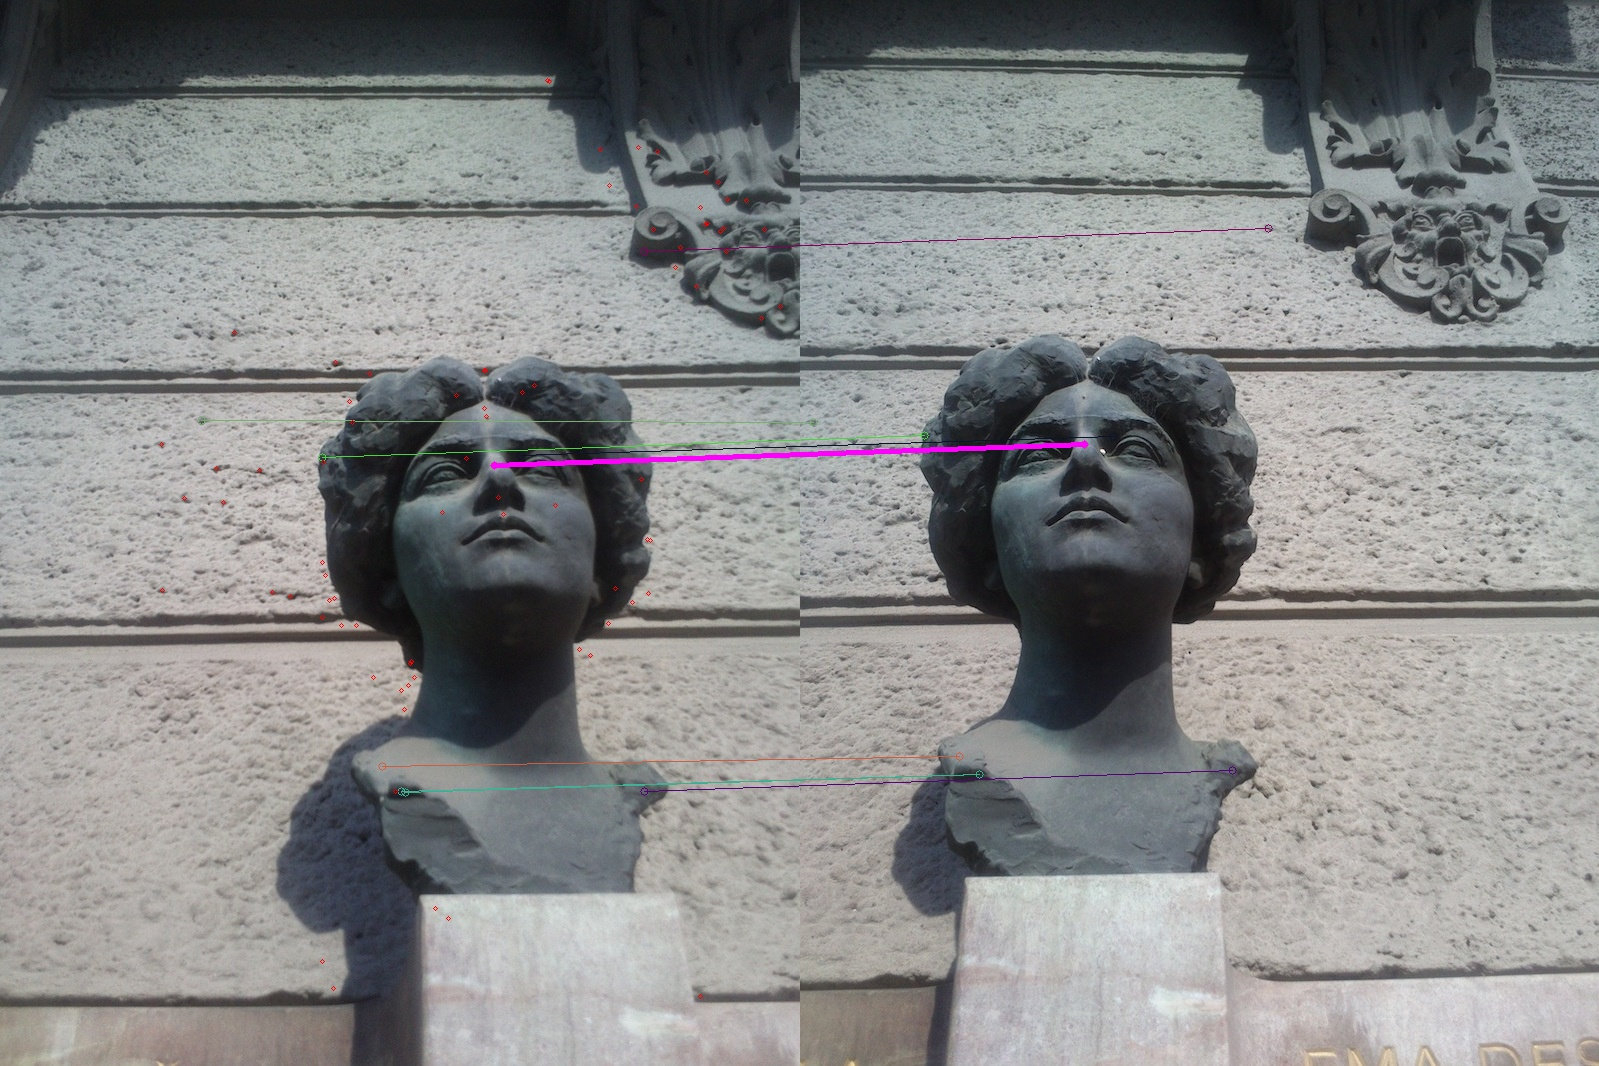
\includegraphics[width=8cm]{img/ema_direction.png}}
% \caption{The most robust match chosen by considering features with large values of the Hessian parameter.}
% \label{fig:robust_match}
% \end{figure}

\subsection{Feature matching}
\label{sec:matching}

Recall that we assume that the two cameras corresponding to our photos differ only by a purely translational movement perpendicular to the principal axis.
In such a case, the epipolar lines corresponding to all positions in one image clearly are parallel lines in the other one. 
Thus, for all pixels in the first image, the position of the corresponding point in the second image differs by a multiple of the displacement vector estimated in the previous step. 
We exploit this now to obtain a large number of SURF correspondences. 

% To find larger number of corresponding point and more information about the scene, we match the detected SURF keypoints one more time in the next step (see Figure \ref{impl2}).
We iterate through all the SURF features in the first image and consider a rectangular region as illustrated on Figure \ref{impl2}.
This rectangle is oriented in the direction of the displacement vector and its center is at the position $\mathbf{x} + \mathbf{d},$ where $\mathbf{x}$ is the original feature's position in the first image and $\mathbf{d}$ is the estimate of the displacement vector from in the previous section. 
Thus, this region corresponds to the most probable position of the corresponding feature. 
Utilizing the buckets described in Section \ref{sec:improving}, we can quickly go through all the second image's features inside the rectangular region. 
We find the feature with the most similar descriptor and consider this to be a putative match.

To avoid mismatches we apply several measures to filter them. 
For example, we accept a match only if there is just one feature with a very similar descriptor and all other feature descriptors we went through are at a distance, say, 20\% bigger than that of the closest match. 
In other words, we accept a match only if the matching feature is a ``clear winner''.
This technique is known as \textit{feature-space outlier rejection}.
To increase stability, we actually employ a second, bigger, rectangle and search for the second closest feature in this bigger one.
We also use the fact that there is orientation assigned to the individual features. 
If our assumptions on the data are correct, then matching features should clearly have nearly identical orientations. 
Therefore, we filter out correspondences where the features have orientations differing by more than a certain threshold. 

%When we know the more accurate relative position of the images, we investigate the keypoints one more time.
%Now we iterate all of them. 
%Each keypoint in the first image we try to match with a keypoint in the estimated corresponding surrounding area in the second image in the shape of oriented rectangle computed based on the more accurate relative image position.
%This oriented rectangle actually consists of two rectangles -- one large and one smaller localised in the middle of the previous one.
%The corresponding keypoint is accepted only if its located in the inner one.
%The size of the larger rectangle is set to 60 $\times$ 120 pixels.
%The inner rectangle after some experiments was set to the 10\% of width and 20\% of height.
%It was shown that it gives better results than only a bit larger window of the the width of 20\% of width and 35\% of height size.
%Matched keypoints which differs too much in the orientation or are not obviously the best match we reject again.
%We can see the comparison in Figure \ref{fig:matching_comparison}.

%Dense correspondence: optical flow::

\subsection{Dense correspondence}

At this point we have relatively robust set of matches, but it is too sparse to visualize directly.
We therefore want to obtain significantly more matches. 
We utilize the optical flow algorithm discussed in Section \ref{sec:optfl} to do this.
The issue now is, however, that optical flow algorithms work well only on pairs of images with very limited visual differences. 
Because of this, we do not run this algorithm on the original image pair.
Rather, for each SURF correspondence we obtain $70 \times 70$ pixel region around the corresponding features and calculate the optical flow between these two feature neighborhoods (see Figure \ref{impl3}).
By calculating the optical flow we get the corresponding points in both photos. 

It is inevitable that the set of SURF correspondences will contain mismatches.
In such a case, the optical flow computation will likely generate almost random values, resulting in significant noise being added to our 3D reconstruction. 
To avoid these, we calculate the variance of the distances between each match.
If the variance is higher than a specified threshold, we discard all of the detected optical flow matches obtained from that particular SURF correspondence.

\section{Graphical visualization}

The result is visualized using OpenGL~ES.
Every correspondence is represented as a triangle in space.
The depth is estimated form the distance of the corresponding pair of features (the smaller the displacement is, the bigger the depth of the point). 
A designated thread is used to render the reconstruction. 
We start rendering when we obtain the first depth information resulting from SURF matching.
Each time new data from a newly executed optical flow calculation are available, we update the model, so that the user can see an animation of the process of execution of our algorithm.

As a result of this approach to visualization, the application seems faster to the user, since the user can see partial results almost immediately after requesting the reconstruction. 

